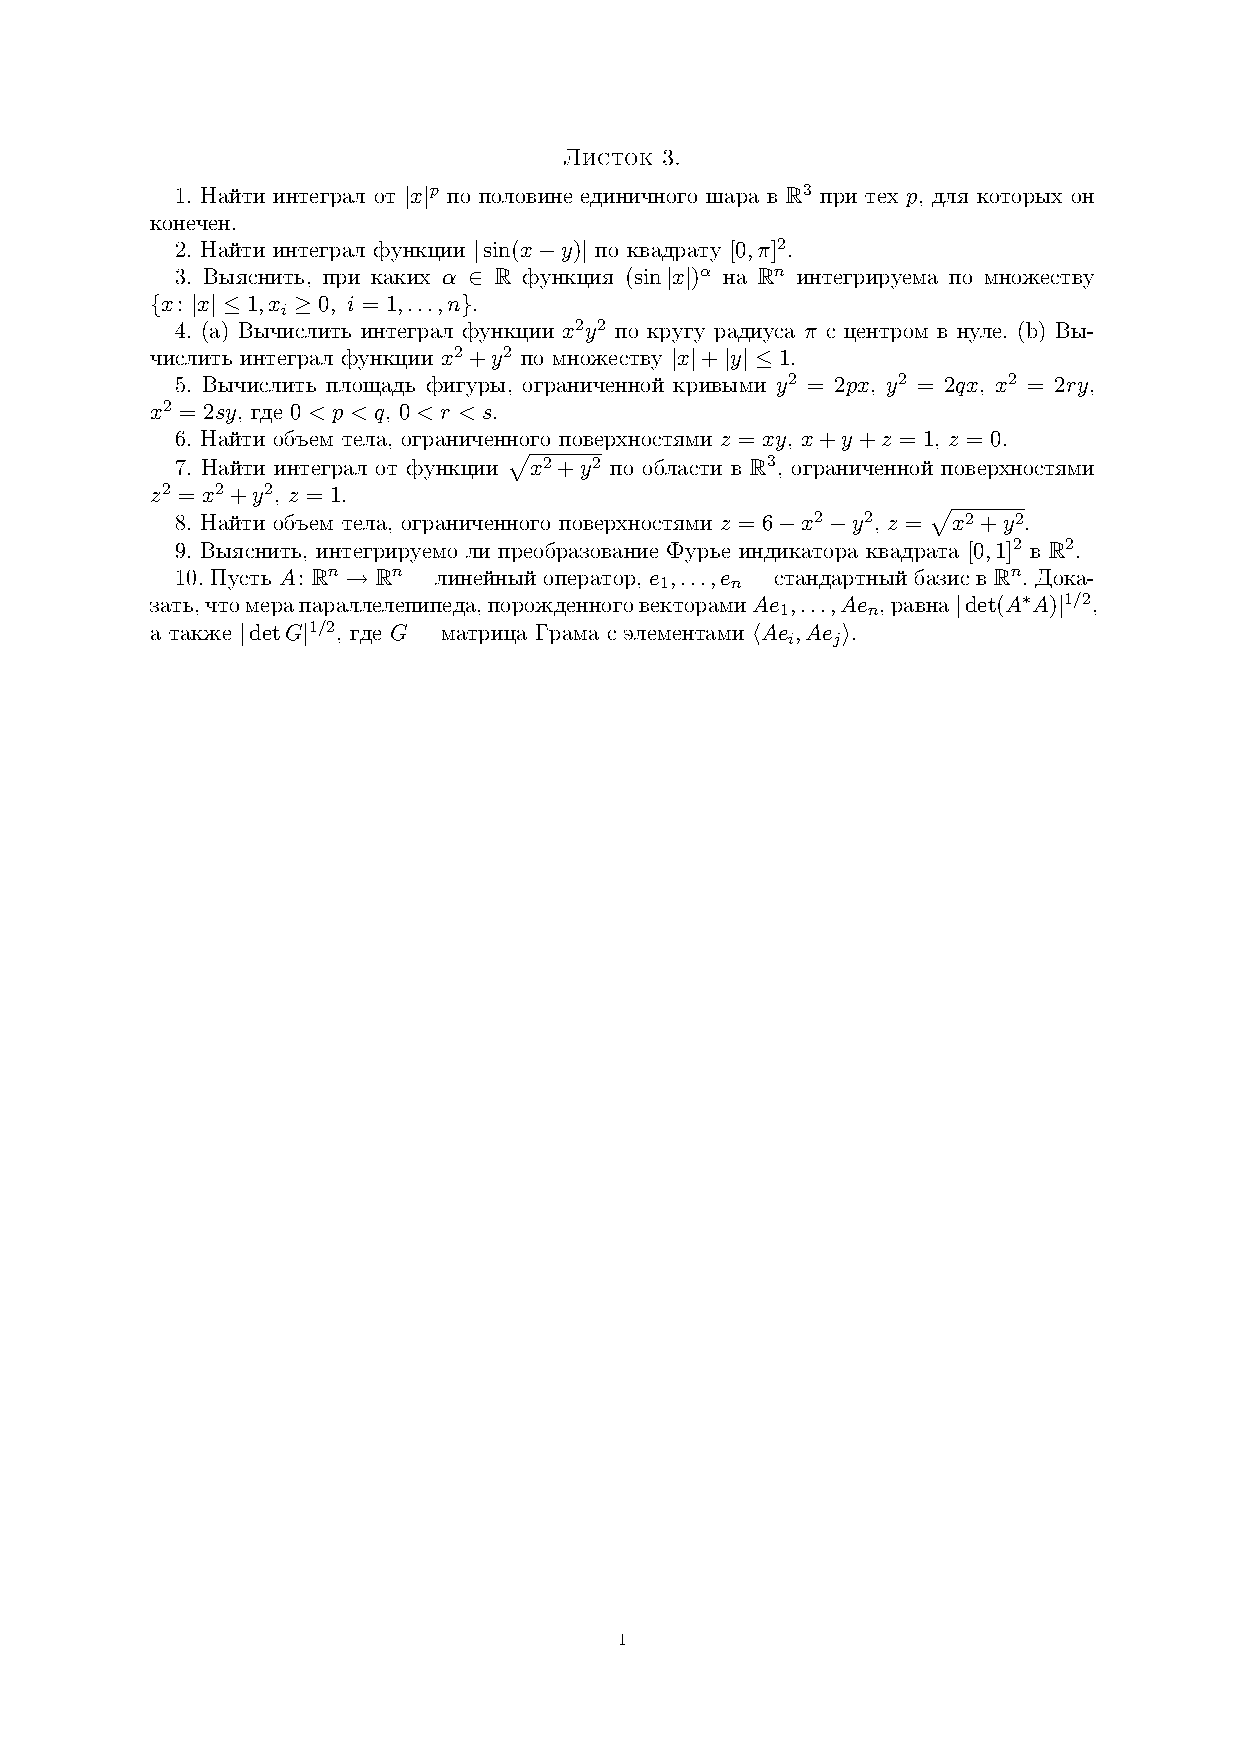
\includepdf[scale=0.95,pages=1,pagecommand=\section*{Условия}]{Tasks/listok-matan3}
\newpage
\section*{Решения}
\subsection*{Задача 1}
	По 5 задаче 2 листка: $\alpha > -3$\\
	Перейдем в сферические координаты
	\begin{gather*}
	\begin{cases}
		x = r \sin(\theta) \cos(\varphi)\qquad \theta \in [0, \pi]\\
		y = r \sin(\theta) \sin(\varphi)\qquad \varphi \in [0, 2\pi)\\
		z = r \cos(\varphi)
	\end{cases}\\
	|J| = r^2 \sin(\theta)\\
	|x| = \sqrt{r^2 \left(\sin^2(\theta) \cos^2(\varphi) + \sin^2(\theta)\sin^2(\varphi) + \cos^2(\theta)\right)} = r\\
	\int_{r \leqslant 1} r^{\alpha} r^2 \sin(\theta) dr d \theta d \varphi =
	\int_{r \leqslant 1} r^{\alpha + 2} dr \int_{0}^{\frac{\pi}{2}} \sin(\theta) d \theta \int_{0}^{2\pi} d \varphi =\\
	\left(\frac{1}{\alpha + 3} r^{\alpha + 3} \bigg|_{0}^{1}\right)\left(-\cos(\theta)\bigg|_{0}^{\frac{\pi}{2}}\right)\left(\varphi \bigg|_{0}^{2\pi}\right) =
	\frac{1}{\alpha + 3} \cdot 2\pi = \frac{2 \pi}{\alpha + 3}
	\end{gather*}
\vskip 0.4in
\begin{comment}
		По 5 задаче 2 листка
	\begin{gather*}
	f(x) = |x|^{\alpha}
	\end{gather*}
	Перейдем в сферические координаты
	\begin{gather*}
	\begin{cases}
	x = r \sin(\theta) \cos(\varphi)\qquad \theta \in [0, \pi]\\
	y = r \sin(\theta) \sin(\varphi)\qquad \varphi \in [0, 2\pi]\\
	z = r \cos(\varphi)
	\end{cases}\\
	|J| = r^2 \sin(\theta)\\
	\int_{r \leqslant 1} (r \sin(\theta) \cos(\varphi))^{\alpha} r^2 \cos(\varphi) dr d \theta d \varphi =
	\int_{0}^{1} r^{\alpha + 2} dr \int_{0}^{\frac{\pi}{2}} (\sin(\theta))^{\alpha} d \theta \int_{0}^{2\pi} (\cos(\varphi))^{\alpha + 1} d  \varphi\\
	\int_{0}^{1} r^{\alpha + 2} dr = \frac{1}{\alpha + 3} r^{\alpha + 3} \bigg|_{0}^{1} = \frac{1}{\alpha + 3}
	\end{gather*}
	Проинтегрируем по частям
	\begin{gather*}
	\int_{0}^{\frac{\pi}{2}} \sin(x)^m dx =
	-\frac{\cos(x)\sin(x)^{m-1}}{m} \bigg|_{0}^{\frac{\pi}{2}} + \frac{m-1}{m} \int_{0}^{\frac{\pi}{2}} \sin^{m-2}(x) dx =
	\frac{m-1}{m}\int_{0}^{\frac{\pi}{2}} \sin^{m-2} (x) dx\\
	\int_{0}^{\frac{\pi}{2}}\sin(x)^m dx = 
	\frac{(m-1)(m-3) \cdot \ldots \cdot 3}{m(m-2) \cdot \ldots \cdot 4} \int_{0}^{\frac{\pi}{2}} \sin(x)^2 dx =
	\frac{(m-1) \cdot \ldots \cdot 3}{m \cdot \ldots \cdot 4} \cdot \frac{\pi}{4}\qquad m \text{ -- четное}\\
	\int_{0}^{\frac{\pi}{2}}\sin(x)^m dx = 
	\frac{(m-1)(m-3) \cdot \ldots \cdot 2}{m(m-2) \cdot \ldots \cdot 3} \int_{0}^{\frac{\pi}{2}} \sin(x)^2 dx =
	\frac{(m-1) \cdot \ldots \cdot 2}{m \cdot \ldots \cdot 3} \cdot \frac{\pi}{4}\qquad m \text{ -- нечетное}
	\end{gather*}
	Аналогичное
	\begin{gather*}
	\int_{0}^{2\pi} \cos(x)^{m} dx =
	\frac{\sin(x)\cos(x)^{m-1}}{m} \bigg|_{0}^{2\pi} + \frac{m-1}{m} \int_{0}^{2\pi} \cos(x)^{m-2} dx\\
	\int_{0}^{\frac{\pi}{2}}\cos(x)^m dx = 
	\frac{(m-1)(m-3) \cdot \ldots \cdot 3}{m(m-2) \cdot \ldots \cdot 4} \int_{0}^{\frac{\pi}{2}} \cos(x)^2 dx =
	\frac{(m-1) \cdot \ldots \cdot 3}{m \cdot \ldots \cdot 4} \cdot \frac{\pi}{4}\qquad m \text{ -- четное}\\
	\int_{0}^{\frac{\pi}{2}}\cos(x)^m dx = 
	\frac{(m-1)(m-3) \cdot \ldots \cdot 2}{m(m-2) \cdot \ldots \cdot 3} \int_{0}^{\frac{\pi}{2}} \cos(x)^2 dx =
	\frac{(m-1) \cdot \ldots \cdot 2}{m \cdot \ldots \cdot 3} \cdot \frac{\pi}{4}\qquad m \text{ -- нечетное}
	\end{gather*}
	В интеграле $(\sin(\theta))^\alpha$ и $(\cos(\varphi))^{\alpha + 1}$ разных четностей
	\begin{gather*}
	\int_{0}^{1} r^{\alpha + 2} dr \int_{0}^{\frac{\pi}{2}} (\sin(\theta))^{\alpha} d \theta \int_{0}^{2\pi} (\cos(\varphi))^{\alpha + 1} d \varphi =\\
	\frac{1}{\alpha + 3} \cdot \frac{(\alpha - 1)(\alpha - 3) \cdot \ldots \cdot 2}{\alpha (\alpha - 2) \cdot \ldots \cdot 3} \cdot \frac{\alpha(\alpha-2) \cdot \ldots \cdot 3}{(\alpha + 1)(\alpha - 1) \cdot \ldots \cdot 4} \cdot \frac{\pi}{4} = \\
	\frac{1}{\alpha + 3} \cdot \frac{2}{\alpha + 1} \cdot \frac{\pi}{4} =
	\frac{\pi}{(\alpha + 3)(\alpha + 1) \cdot 2}
	\end{gather*}
\end{comment}

\subsection*{Задача 2}
	\begin{gather*}
	\int_{0}^{\pi} \int_{0}^{\pi} |\sin(x-y)| dxdy = 2\pi\\
	\int_{0}^{\pi} |\sin(x-y)| dx = \int_{0}^{\pi} (\sin(x))dx = \cos(x) \bigg|_{0}^{\pi} = 2
	\end{gather*}
	Так как период $|\sin(x)| = \pi$, то интеграл по отрезку длиной $\pi$ равен $\forall \text{const} = y$
	\begin{gather*}
	\int_{0}^{\pi} |\sin(x-y)| = \int_{0}^{\pi} \sin(x) dx\\
	\int_{0}^{\pi} 2 dy = 2y \bigg|_{0}^{\pi} = 2\pi
	\end{gather*}
\vskip 0.4in


\subsection*{Задача 3}
	Перейдем в сферические координаты
	\begin{gather*}
	\begin{cases}
		x_1 = r \cos(\theta_1)\\
		x_2 = r \sin(\theta_1) \cos(\theta_2)\\
		\vdots\\
		x_{n-1} = r \sin(\theta_1) \ldots \sin(\theta_{n-2}) \cos(\theta_{n-1})\\
		x_n = r \sin(\theta_1) \ldots \sin(\theta_{n-2}) \sin(\theta_{n-1})
	\end{cases}
	\qquad \theta_1,\ldots,\theta_{n-2} \in [0,\pi]\quad \theta_{n-1} \in [0,2\pi)\\
	|J| = r^{n-1} f(\theta_1,\ldots, \theta_{n-1})\\
	u = \{x:\ r \leqslant 1,\ \theta_1,\ldots,\theta_{n-2} \in [0, \frac{\pi}{2}],\ \theta_{n-1} \in [0, \pi]\}\\
	\int_{u}(\sin(r))^{\alpha} r^{n-1} f(\theta_1,\ldots,\theta_{n-1}) dr d\theta_1 \ldots d\theta_{n-1}\\
	(\sin(r))^{\alpha} r^{n-1} = \left(r - \frac{r^3}{3!} + \ldots \right)^{\alpha} r^{n-1} = r^{\alpha + n - 1} + \ldots
	\end{gather*}
	$r \leqslant 1$ тогда если $\int r^{\alpha + n - 1} dr < \infty$ то $(\sin r)^{\alpha} < \infty$ и $\alpha + n - 1 > -1$, то есть $\alpha > -n$
\vskip 0.4in


\subsection*{Задача 4}
\begin{enumerate}
\item[(a)] 
	\begin{gather*}
		f(x,y) = x^2y^2\\
		\begin{cases}
			x = r \sin(\varphi)\\
			y = r \cos(\varphi)
		\end{cases}
		\qquad |J| = r
	\end{gather*}
	Перейдем от двойного интеграла к повторному
	\begin{gather*}
		S =
		\iint_{U} x^2 y^2 dx dy =\\
		\int_{0}^{2\pi} d \varphi \int_{0}^{\pi} r^2 \cos(\varphi)^2 r^2 \sin(\varphi)^2 rdr =
		\int_{0}^{2\pi} d \varphi \left(\cos(\varphi)^2 \sin(\varphi)^2 \frac{r^6}{6}\right)\bigg|_{0}^{\pi} =\\
		\int_{0}^{2\pi} \frac{\pi^6}{6} \cos(\varphi)^2 \sin(\varphi)^2 d \varphi =
		\frac{\pi^6}{6} \left(\frac{1}{8}\varphi - \frac{\sin(4\varphi)}{32}\right)\bigg|_{0}^{2\pi} = \frac{\pi^7}{24}
	\end{gather*}
\item[(b)] 
	\begin{gather*}
		f(x,y) = x^2 + y^2\qquad S = \{(x,y):\ |x| + |y| \leqslant 1\}\\
		\iint_{S} (x^2 + y^2) dxdy = 4\iint_{\substack{x,y \geqslant 0 \\ x+y \leqslant 1}} (x^2 + y^2)dxdy =\\
		4\int_{0}^{1} dx \int_{0}^{1-x} (x^2 + y^2) dy = 4\int_{0}^{1} dx (x^2y + \frac{y^3}{3})\bigg|_{0}^{1-x} =\\
		4\int_{0}^{1} \left(x^2(1-x) + \frac{(1-x)^3}{3}\right) dx = 4 \int_{0}^{1} (x^2 - x^3 + \frac{1}{3} - x + x^2 - \frac{x^3}{3}) dx =\\
		4\left(\frac{1}{3} - \frac{1}{4} + \frac{1}{3} - \frac{1}{2} + \frac{1}{3} - \frac{1}{12}\right) = \frac{2}{3}
	\end{gather*}
\end{enumerate}
\vskip 0.4in


\newpage
\subsection*{Задача 5}
	\begin{figure}[!h]
		
\includegraphics[width=0.7\linewidth]{Pic3}
	\end{figure}
	\vskip 0.2in
	Заметим что рассматриваемая фигура -- четырехвершинник, сторонами которого являются параболы. Тогда мы можем заметить, что его вершины -- точки пересечения парабол, то есть
	\begin{gather*}
		\begin{cases}
			y^2 = 2ax\\
			x^2 = 2by
		\end{cases}\qquad
		(x,y) = \left(2\sqrt[3]{a b^2}, 2\sqrt[3]{a^2 b}\right)
	\end{gather*}
	То есть вершины это $\alpha_{1} = \left(2\sqrt[3]{p r^2}, 2\sqrt[3]{p^2 r}\right),\ \alpha_{3} = \left(2\sqrt[3]{p s^2}, 2\sqrt[3]{p^2 s}\right),\ \alpha_{2} = \left(2\sqrt[3]{q r^2}, 2\sqrt[3]{q^2 r}\right),\ \alpha_{4} = \left(2\sqrt[3]{q s^2}, 2\sqrt[3]{q^2 s}\right)$. Тогда
	\begin{gather*}
		S_1 =
		\int_{\beta_1}^{\beta_2} \int_{x_1}^{y_1} dy dx = 
		\int_{2\sqrt[3]{pr^2}}^{2\sqrt[3]{qr^2}} \int_{\sqrt{2px}}^{\frac{x^2}{2r}} dy dx =\\
		\int_{2\sqrt[3]{pr^2}}^{2\sqrt[3]{qr^2}} \left(\frac{x^2}{2r} - \sqrt{2px}\right)dx =
		\left(\frac{x^3}{6r} - \frac{2}{3}x \sqrt{2px} \right) \bigg|_{2\sqrt[3]{pr^2}}^{2\sqrt[3]{qr^2}} =\\
		\frac{4}{3} r(q-p) - \frac{8}{3}r \sqrt{pq} + \frac{8}{3} pr\\
		\\
		S_2 = 
		\int_{\beta_2}^{\beta_3} \int_{x_1}^{x_2} dy dx =
		\int_{2\sqrt[3]{qr^2}}^{2\sqrt[3]{ps^2}} \int_{\sqrt{2px}}^{\sqrt{2qx}} dy dx =\\
		\int_{2\sqrt[3]{qr^2}}^{2\sqrt[3]{ps^2}} \sqrt{2qx} - \sqrt{2px} dx =
		\frac{2}{3}(\sqrt{2qx^3} - \sqrt{2px^3})\bigg|_{2\sqrt[3]{qr^2}}^{2\sqrt[3]{ps^2}} =
		\frac{8}{3}(s\sqrt{pq} - ps - qr + r\sqrt{pq})\\
		\\
		S_3 =
		\int_{\beta_3}^{\beta_4} \int_{y_2}^{x_2} dy dx =
		\int_{2\sqrt[3]{ps^2}}^{2\sqrt[3]{qs^2}} \sqrt{2qx} - \frac{x^2}{2s} dx =\\
		\frac{2}{3} \sqrt{2qx^3} - \frac{x^3}{6s} \bigg|_{2\sqrt[3]{qs^2}}^{2\sqrt[3]{ps^2}} =
		\frac{8}{3}(s\sqrt{pq} - \sqrt{qps^2}) - \frac{4}{3}(qs - ps)\\
		\\
		S_1 + S_2 + S_3 =
		\frac{4}{3}r(q-p) - \frac{8}{3}r\sqrt{pq} + \frac{8}{3}pr + \frac{8}{3}(s\sqrt{pq} - ps - qr + r\sqrt{pq}) + \frac{8}{3}(qs - s\sqrt{qp}) - \frac{4}{3}(qs - ps) = \\
		-\frac{4}{3}rq + \frac{4}{3}pr - \frac{4}{3}ps + \frac{4}{3}qs = 
		\frac{4}{3}(q-p)(s-r)
	\end{gather*}
\vskip 0.4in


\newpage
\subsection*{Задача 6}
	\begin{figure}[!h]
		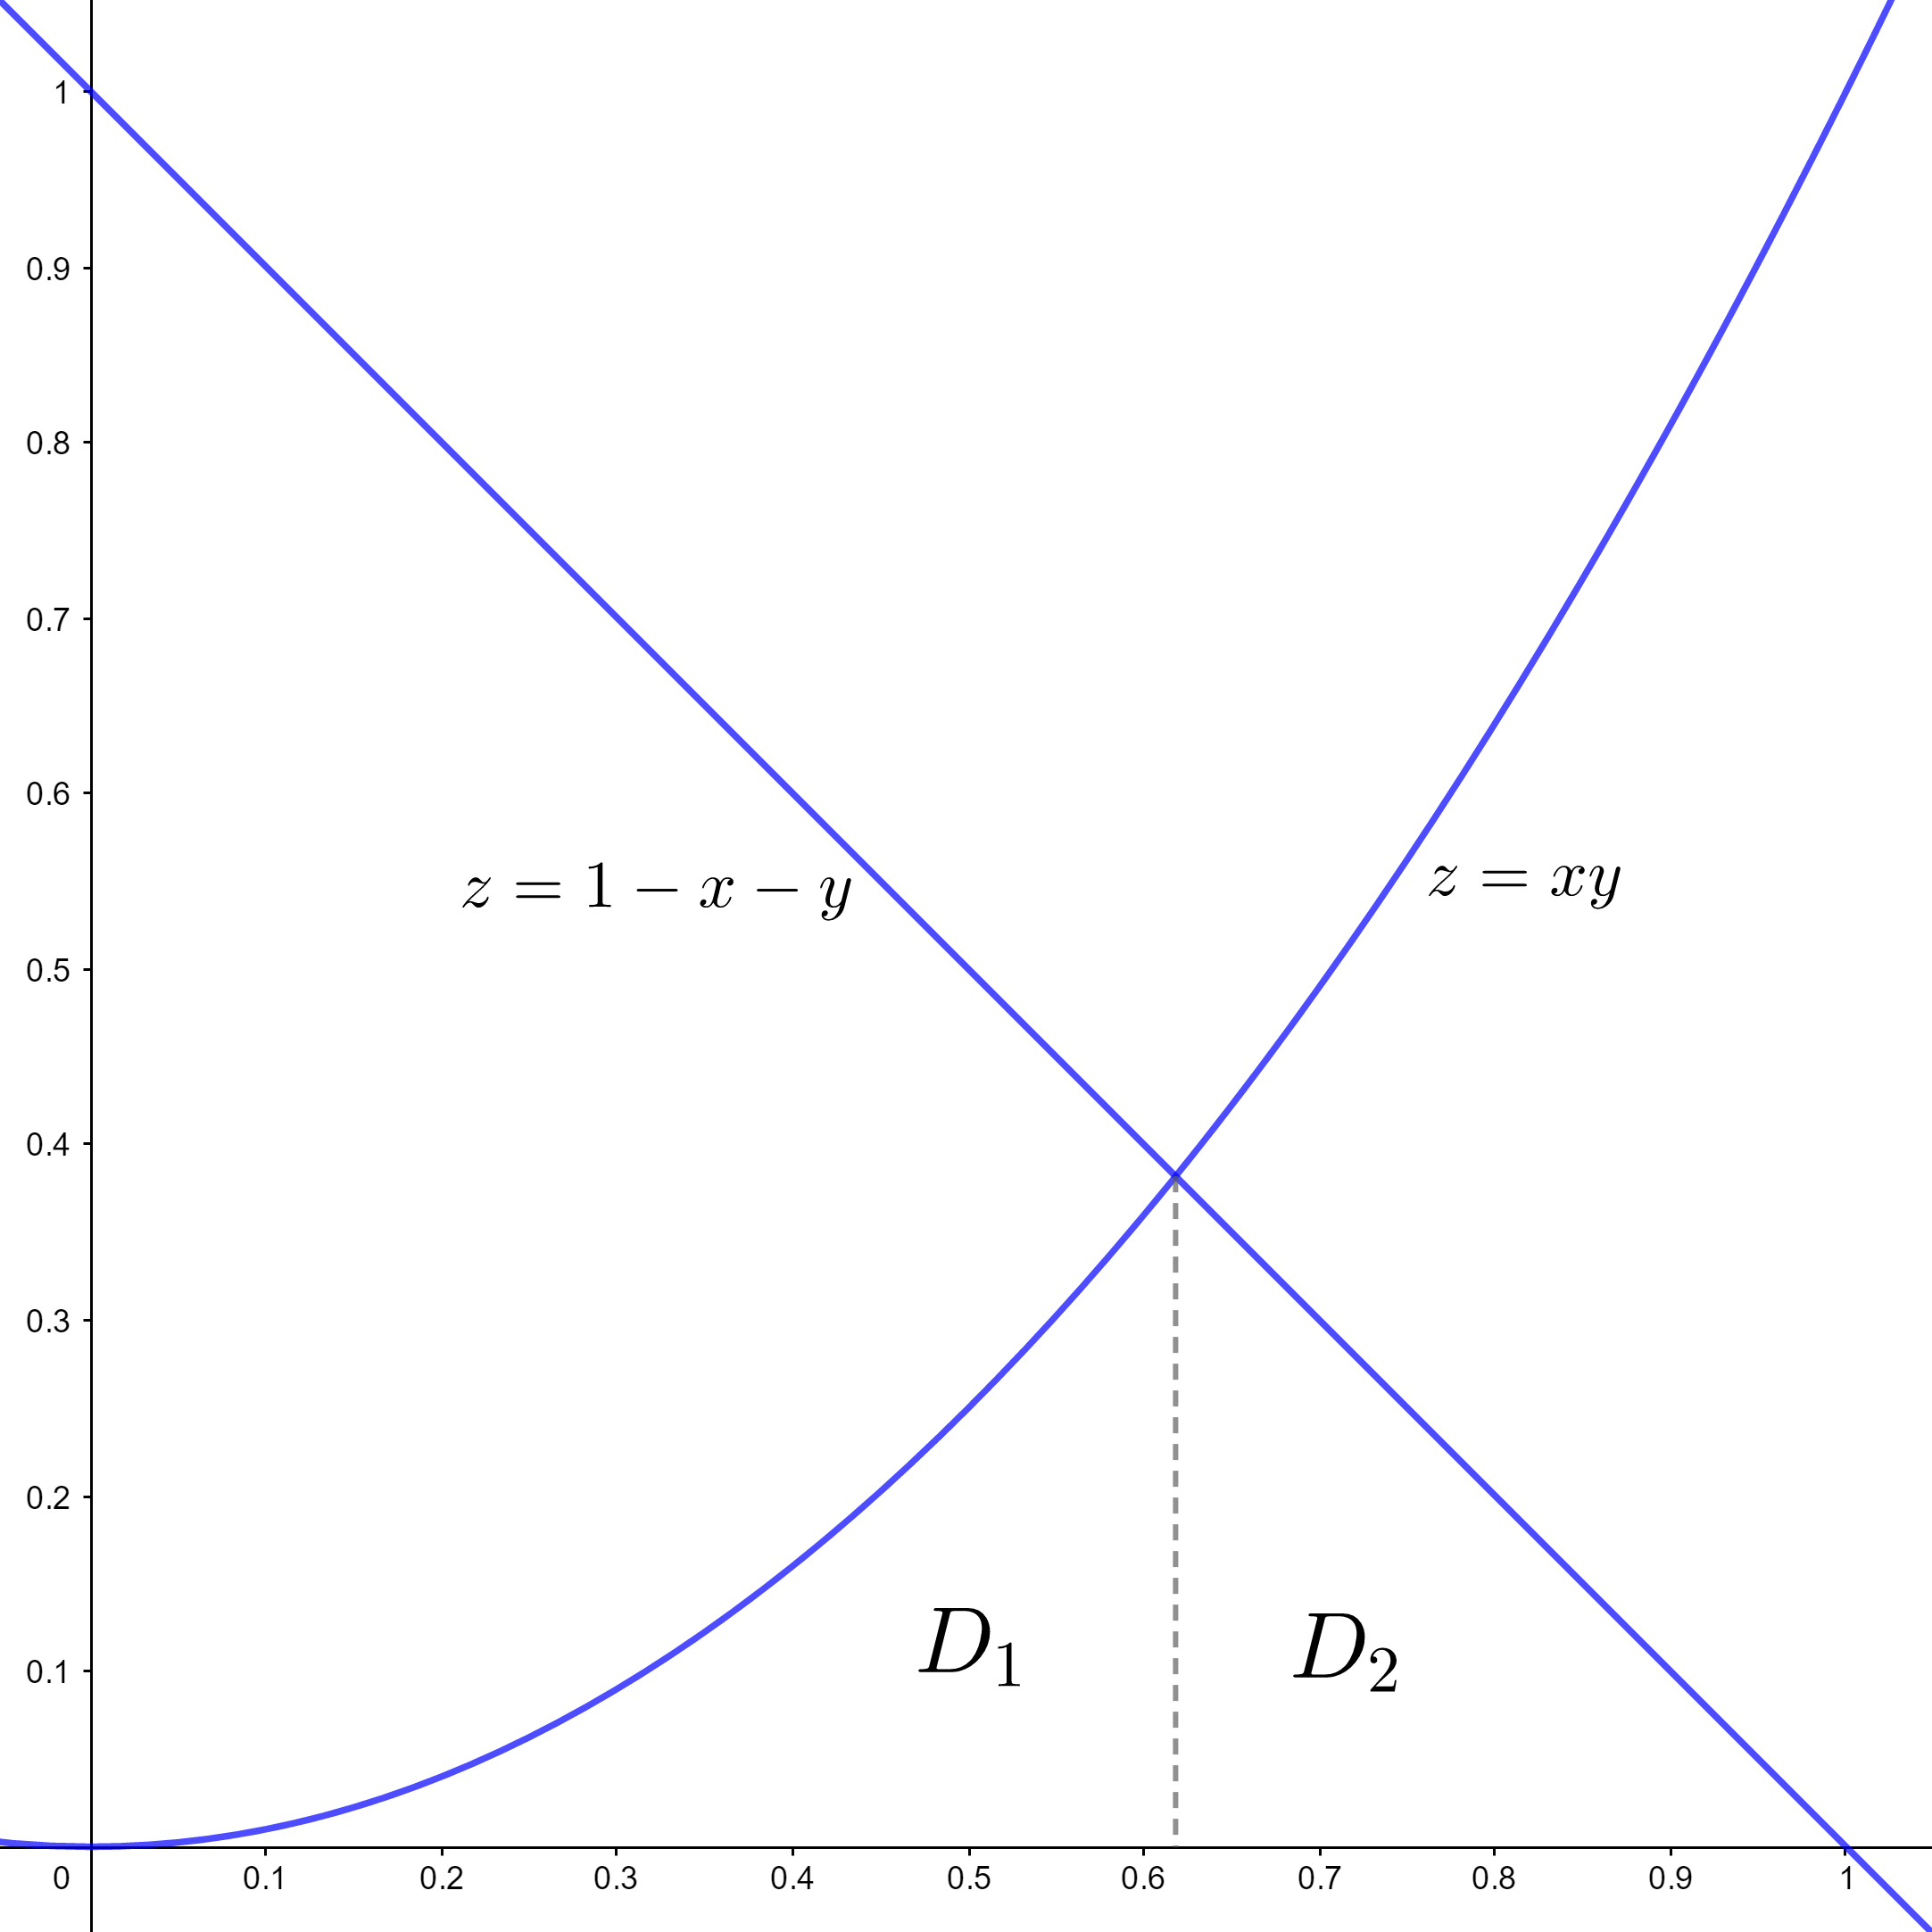
\includegraphics[width=0.4\linewidth]{Pic4}
	\end{figure}
	\vskip 0.2in
	Найдем точки пересечения
	\begin{gather*}
	\begin{cases}
	z = xy\\
	x+y+z = 1
	\end{cases}
	\qquad
	x+y+xy = 1\quad y = \frac{1-x}{1+x}\\
	\begin{cases}
	x+y+z = 1\\
	z = 0
	\end{cases}
	\qquad
	x+y = 1
	\end{gather*}
	Тогда
	\begin{gather*}
	V = D_1 + D_2 = \int_{0}^{1} dx \int_{\frac{1-x}{1+x}}^{1-x} dy \int_{0}^{1-x-y} dz + \int_{0}^{1} dx \int_{0}^{\frac{1-x}{1+x}} dy \int_{0}^{xy} dz =\\
	\int_{0}^{1} \left(y - xy - \frac{1}{2}y^2 \bigg|_{\frac{1-x}{1+x}^{1-x}}\right)dx + \int_{0}^{1} \left(\frac{1}{2}xy^2\bigg|_{0}^{\frac{1-x}{1+x}}\right) dx =\\
	\int_{0}^{1} \left(1 - x - \frac{1-x}{1+x} - x(1-x) + x \frac{1-x}{1+x} - \frac{1}{2}(1-x)^2 + \frac{1}{2} \left(\frac{1-x}{1+x}\right)^2\right)dx + \int_{0}^{1} \left(\frac{1}{2} \cdot \frac{(1-x)^2}{(1+x)^2}\right) dx
	\end{gather*}
	Заметим что
	\begin{gather*}
	-\frac{(1-x)}{(1+x)}(1-x) + (1-x)(1-x) + \frac{1}{2}(1-x)^2 \left(\frac{1}{(1+x)^2} - 1\right) =\\
	(1-x)^2 \left(-\frac{1}{1+x} + \frac{1}{2} + \frac{1}{2} \cdot \frac{1}{(1+x)^2}\right) =
	(1-x)^2 \left(\frac{1}{\sqrt{2}(1+x)} - \frac{1}{\sqrt{2}}\right)^2 =
	\frac{(1-x)^2 x^2}{2(1+x)^2}
	\end{gather*}
	Тогда
	\begin{gather*}
	\int_{0}^{1} \frac{(1-x)^2 x^2}{2(1+x)^2} dx + \int_{0}^{1} \frac{(1-x)^2 x}{2(1+x)^2} dx =\\
	\frac{1}{2} \int_{0}^{1} \left(\frac{1-x}{1+x}\right)^2 (x+1) dx =\\
	\frac{1}{2} \int_{0}^{1} \frac{(1-x)^2 x}{1+x} dx =\\
	\frac{1}{2} \int_{0}^{1} (x^2 - 3x + 4 - \frac{4}{x+1}) dx =\\
	\frac{1}{2} \left(\frac{1}{3}x^3 - \frac{3}{2}x^2 + 4x - 4\ln(x+1)\right)\bigg|_{0}^{1} =\\
	\frac{1}{2} \left(\frac{1}{3} - \frac{3}{2} + 4 - 4\ln(2)\right) =\\
	\frac{17}{12} - 2\ln(2)
	\end{gather*}
\vskip 0.4in
\begin{comment}
Найдем точки пересечения
\begin{gather*}
z = xy \text{ и } z = 0\\
xy = 0\ \Rightarrow\ x = 0 \text{ или } y = 0\\
\\
x + y + z = 1 \text{ и } z = 0\\
x + y = 1\ \Rightarrow\ x \geqslant 0\quad y \leqslant 1\\
\\
z = xy \text{ и } x + y + z = 1\\
1-x-y = xy\ \Rightarrow\ y = \frac{1-x}{1+x}\quad z = x \cdot \frac{1-x}{1+x}
\end{gather*}
Тогда
\begin{gather*}
V = \int_{0}^{1} \int_{0}^{1} \int_{0}^{x \cdot \frac{1-x}{1+x}} dzdxdy =
\int_{0}^{1} \int_{0}^{1} 2-x+\frac{2}{1+x} dxdy =\\
\int_{0}^{1} 2x - \frac{1}{2} x^2 + 2\ln(x + 1) \bigg|_{0}^{1} dy=
\int_{0}^{1} \frac{3}{2} + 2\ln(2) dy = \frac{3}{2} + 2 \ln(2)
\end{gather*}
\end{comment}

\subsection*{Задача 7}
	\begin{gather*}
	\begin{cases}
		z^2 = x^2 + y^2\\
		z = 1
	\end{cases}\qquad
	x^2 + y^2 = 1
	\end{gather*}
	Перейдем к цилиндрическим координатам
	\begin{gather*}
	\begin{cases}
		x = \rho \cos(\phi)\\
		y = \rho \sin(\phi)\\
		z = z
	\end{cases}
	\ \Rightarrow\ 
	f = \rho,\ z^2 = \rho^2,\ z=1
	\ \Rightarrow\ 
	\rho \in [0,1],\ z \in [0,1]
	\end{gather*}
	Тогда
	\begin{gather*}
	\begin{aligned}
		V & = \int_{0}^{1} \int_{0}^{2\pi} \int_{0}^{1} f(\rho) \rho d \rho d \phi dz\\
		& = \int_{0}^{1} \int_{0}^{2\pi} \frac{\rho^3}{3} \bigg|_{0}^{z} d \phi dz\\
		& = \int_{0}^{1} \int_{0}^{2\pi} \frac{z^3}{3} d \phi dz\\
		& = \int_{0}^{1} \frac{2\pi}{3} z^3 dz\\
		& = \frac{\pi z^4}{6} \bigg|_{0}^{1}
		& = \frac{\pi}{6}
	\end{aligned}
	\end{gather*}
\vskip 0.4in


\subsection*{Задача 8}
	Рассмотрим точки пересечения: $6 - x^2 - y^2 = \sqrt{x^2 + y^2},\ (x,y) = (2,2)$, обозначим $x^2 + y^2 = r^2$, тогда
	\begin{gather*}
		6 - r^2 = r\qquad r^2 + r - 6 = 0\qquad r_1 = 2,\ r_2 = -3
	\end{gather*}
	Тогда $z = \sqrt{x^2 + y^2} = \sqrt{r^2} = 2$.\\
	Перейдем к цилиндрическим координатам $x^2 + y^2 = r^2$ и $dxdydz = rdrd\phi dz$ и
	\begin{gather*}
	\begin{aligned}
		V & = \iiint_U r dr d\phi dz\\
		& = \int_{0}^{2} \int_{0}^{2\pi} \int_{r}^{6 - r^2} r d\phi dz dr\\
		& = \int_{0}^{2} \int_{0}^{2\pi} rz \bigg|_{r}^{6-r^2} d\phi dr\\
		& = \int_{0}^{2} \int_{0}^{2\pi} 6r-r^3-r^2 d\phi dz\\
		& = \int_{0}^{2} 2\pi(6r-r^3-r^2) dr\\
		& = 2\pi (3r^2 - \frac{r^4}{4} - \frac{r^3}{3}) \bigg|_{0}^{2}\\
		& = 2\pi (12-4-\frac{8}{3})
		& = 2\pi \cdot \frac{16}{3}
		& = \frac{32}{3}\pi
	\end{aligned} 
	\end{gather*}
\vskip 0.4in


\subsection*{Задача 9}
	\begin{gather*}
	\hat{I}(u,v) =\frac{1}{\sqrt{2\pi}^2} \int_{\mathbb{R}^2} e^{-i(xu + yv)} I dxdy =\\
	\frac{1}{2 \pi} \int_{\mathbb{R}} e^{-iyv} I_2 dy \int_{\mathbb{R}} e^{-ixu} I_1 dx =\\
	\frac{1}{2 \pi} \int_{0}^{1} e^{-iyv} dy \int_{0}^{1} e^{-ixu} dx\\
	\\
	\int_{\mathbb{R}} e^{-ixu} I_1 = \int_{0}^{1} e^{-ixu} I_1 dx\qquad \text{так как на остальных интервалах функция зануляется}\\
	\int_{\mathbb{R}^2} \hat{I} dudv =\\
	\frac{1}{2 \pi} \int_{\mathbb{R}} \left(\int_{0}^{1} e^{-iyv} dy\right)dv \int_{\mathbb{R}} \left(\int_{0}^{1} e^{-ixu} dx\right)du\\
	\frac{e^{-ixu}}{-iu} \bigg|_{0}^{1} = \frac{i}{u} (e^{-iu} + 1)\\
	\int_{\mathbb{R}} \left(\frac{i}{n} + i \frac{e^{-iu}}{u}\right) du =
	i \left(\int_{-\infty}^{\infty} \frac{du}{u} + \int_{-\infty}^{\infty} \frac{e^{-iu}}{u} du\right) =
	\int_{-\infty}^{\infty} \frac{\sin(u)}{u} + i \left(\int_{-\infty}^{\infty} \frac{du}{u} + \int_{-\infty}^{\infty} \frac{\cos(u)}{u} du\right)
	\end{gather*}
	Заметим что факту существования этого интеграла равносилен тому, что $\frac{\sin(u)}{u}$ и $\frac{du}{u} + \frac{\cos(u)}{u} du$ интегрируемы\\
	$\int_{-\infty}^{\infty} \frac{\sin(u)}{u} du$ интегрируема $\Leftrightarrow\quad \left|\frac{\sin(x)}{x}\right|$ интегрируема (по Лебегу)
	\begin{gather*}
	\int_{-\infty}^{\infty} \left|\frac{\sin(x)}{x}\right| dx =
	\int_{-\infty}^{0} \left|\frac{\sin(x)}{x}\right| dx + \int_{0}^{\infty} \left|\frac{\sin(x)}{x}\right| dx =
	\int_{-\infty}^{0} -\frac{|\sin(x)|}{x} dx + \int_{0}^{\infty} \frac{|\sin(x)|}{x} dx =\\
	\sum_{n = 0}^{\infty} \int_{\pi n}^{\pi(n + 1)} \frac{|\sin(x)|}{x} dx + \sum_{n = 0}^{\infty} \int_{-\pi(n+1)}^{-\pi n} -\frac{|\sin(x)|}{x} dx =\\
	\sum_{n = 0}^{\infty} \int_{0}^{\pi} \frac{|\sin(x - \pi n)|}{(x - \pi n) + \pi n} d(x - \pi n) +
	\sum_{n = 0}^{\infty} \int_{0}^{\pi} -\frac{|\sin(x + \pi(n+1))|}{(x + \pi(n+1)) - \pi(n+1)} d(x + \pi(n+1)) =\\
	2\sum_{n = 0}^{\infty} \int_{0}^{\pi} \frac{|\sin(x - \pi n)|}{(n+1)\pi} d(x - \pi n) =\\
	2 \int_{0}^{\pi} |\sin(x - \pi n)| d(x - \pi n) \cdot \sum_{n = 0}^{\infty} \frac{1}{\pi (n+1)} = 2 \frac{2}{\pi} \sum_{n = 0}^{\infty} \frac{1}{n+1} = \infty
	\end{gather*}
	\vskip 0.1in
	TL;DR\\
	Можно прочитать про интеграл Дирихле, он не является абсолютно сходящимся, а следовательно $\left|\frac{\sin(x)}{x}\right|$ не интегрируется по Лебегу
	\vskip 0.2in
	Значит $\int_{-\infty}^{\infty} \left|\frac{\sin(x)}{x}\right| dx = \infty$, то есть $\int_{\mathbb{R}} \left(\int_{0}^{1} e^{-iux} dx\right) du$ не существует, а следовательно и интеграл преобразования Фурье тоже не существует
\vskip 0.4in

\begin{comment}
\begin{gather*}	
A = [0,1]^2\\
I_A = 
\begin{cases}
1\quad (x,y) \in A\\
0\quad (x,y) \notin A
\end{cases}\qquad \text{ в } \mathbb{R}^2\\
I_A = I_x I_y\qquad x = [0,1]\in O_x\quad y = [0,1]\in O_y
\hat{f}(\lambda, \mu) = 
\iint_{\mathbb{R}^2} e^{-i \lambda x - i \mu y} I_A dxdy =
\int_{\mathbb{R}} e^{-i \lambda x} I_x dx \int_{\mathbb{R}} e^{-i \mu y} I_y dy\\
\sin(x) = \frac{e^{ix} - e^{-ix}}{2i}\\
\cos(x) = \frac{e^{ix} + e^{-ix}}{2}\\
\int_{\mathbb{R}} e^{-i \lambda x} I_x dx = 
\int_{-\infty}^{0} e^{-i \lambda x} I_x dx + \int_{0}^{1} e^{-i \lambda x} I_x dx + \int_{1}^{\infty} e^{-i \lambda x} I_x dx =\\
\int_{0}^{1} e^{-i \lambda x} dx = 
\frac{1}{-i \lambda} e^{-i \lambda x} \bigg|_{0}^{1} =
\frac{e^{-i \lambda} - 1}{-i \lambda} \text{ интегрируемо }\\
\hat{f}(\lambda, \mu) = \frac{(e^{-i \lambda} - 1)(e^{-i \mu} - 1)}{\lambda \mu}
\end{gather*}
\end{comment}

\subsection*{Задача 10}
	Объем параллелепипеда, натянутого на векторы $x_1, \ldots, x_n$ -- определитель матрицы с соответствующими столбцами. Теперь посмотрим на меру. У единичного параллелепипеда это 1, а теперь мы проводим замену переменных, домножая их на А. Тогда подынтегральное выражение домножится на матрицу перехода, то есть на А и мера будет равна $|\det(A^* A)|^{\frac{1}{2}}$. Определитель транспонированной матрицы равен определителю обычной матрицы, а матрица Грама это произведение обычной с транспонированной, откуда $A^* A = G$ и $|\det G|^{\frac{1}{2}} = |\det A^* A|^{\frac{1}{2}}$.
\begin{comment}
При умножении базисных векторов на $A$, параллелепипед будет иметь меру $\det A$. При замене координат происходит то же самое (подынтегральное выражение умножится на определитель матрицы переход $\det A$), осталось заметить, что $\det A = \det A^t$ и $\det G = \det A^t \cdot \det A$
\end{comment}
